\section{Experiments}
Measuring the quality of the TweetRank score is difficult because there are no reference corpora to be tested on, the only thing that we did was to try it together with Solr and check that the results quality was good.

We also plotted the sorted list of TweetRank values in log-log scale and checked that it follows closely the power law, as it was stated by \cite{Avrachenkov:2007:MCM:1272804.1272825}. Figure \ref{fig:tweetrank_powerlaw} shows this fact.

\begin{figure}
\centering
\subfigure[Sorted TweetRank, loglog scale]{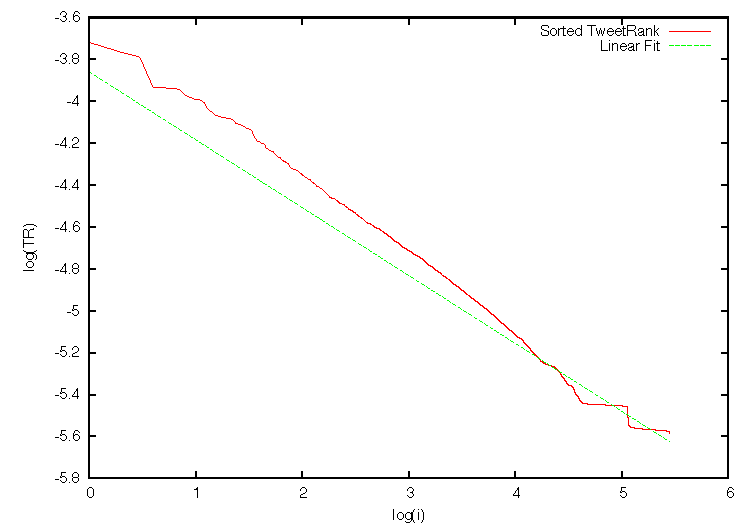
\includegraphics[width=0.4\textwidth]{tweetrank_powerlaw.pdf}\label{fig:tweetrank_powerlaw}}
\qquad
\subfigure[Number of tweets vs. running time]{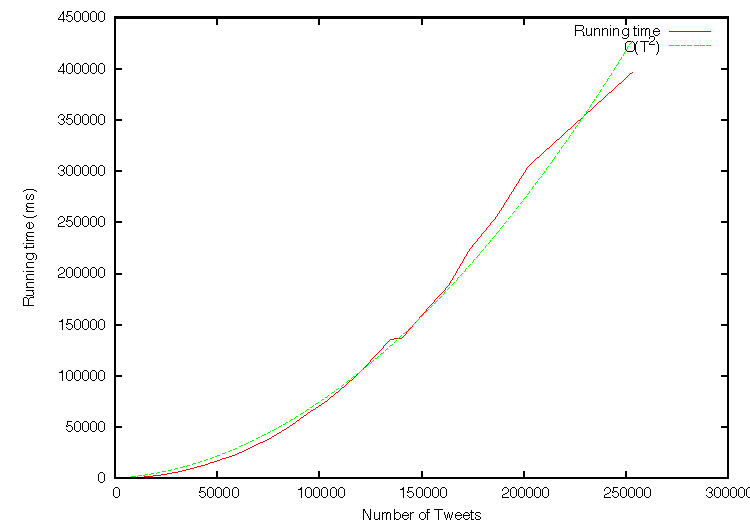
\includegraphics[width=0.4\textwidth]{tweetrank_times.pdf}\label{fig:tweetrank_times}} 
\caption{Experiment results}
\end{figure}

Figure \ref{fig:tweetrank_times} shows the number of tweets versus the running time. We see that a quadratic curve fits very well with the experimental data, which confirms our analysis of the expected running time described in equation \ref{eq:running_time} (section \ref{sec:tweetrank_implementation}). These results were obtained on a machine and parameters specified in table \ref{table:machine_spec}. 
\begin{table}
\centering
\begin{tabular}{|c|c|}
\hline Processor & Intel Core i5, 2 cores at 2.4GHz, 64 bits \\
\hline Memory & Main: 4GB DDR3, Cache L3: 3MB, Cache L2: 256KB \\
\hline OS &  Mac OS X 10.6.8 Snow Leopard \\
\hline Compiler & javac 1.6.0\_31, 64 bits, no optimization parameters \\
\hline Others & 8 threads, $\alpha = 0.2, \beta = 0.4, \gamma = 0.2, \delta = 0.04, \epsilon = 0.16, \zeta = 0.2, M = T/100$ \\
\hline
\end{tabular}
\caption{Specification of the machine used for experimentation}
\label{table:machine_spec}
\end{table}

It's important to observe that our model has many parameters to be adjusted. Design a good set of experiments to choose the best values would require a lot of time and also lot of time to be tested. For estimating the optimal values for the probabilities used by our algorithm, the simplest solution would be trying different combinations of their values and try to find the one that produces better results. However, this would require a tremendous amount of time and, even more important, would require a labelled dataset to measure the precision and recall of the search engine.

An other approach, would be monitor those probabilities on real users. For example, installing a plug-in on the web browser that registers the activity of the user (when the user clicks on a retweet or reply, on a mentioned user, on the friends list, etc). To preserve anonymity, this would be a plug-in installed in volunteer's browsers and the data collected would not contain any personal information (it is not important for us which tweet is viewing the user, but how he or she got to it). Using this data, one could estimate those probabilities and use the estimated value to compute the TweetRank.